\documentclass[11pt,a4pape,dvipdfmx]{jarticle}
\title{Bayesian Data Analysis\\Andrew Gelman, John B.Carlin, Hal S.Stern,\\David B.Dunson, Aki Vehtari, and Donald B.Rubin}

\setlength{\oddsidemargin}{0cm}
\setlength{\evensidemargin}{0cm}
\setlength{\topmargin}{-1.8cm}
\setlength{\textheight}{25cm}
\setlength{\textwidth}{16cm}

\usepackage[dvipdfmx]{hyperref}
\usepackage{listings,jlisting}
\usepackage{slashbox}
\usepackage{ascmac}
\usepackage{amsmath}
\usepackage[dvipdfmx]{graphicx}
\usepackage{float}
\usepackage{newtxtext,newtxmath}
\usepackage{graphicx}
\usepackage{color}
\usepackage{url}
\usepackage{bm}
\usepackage{listings,jlisting}
\usepackage{slashbox}
\usepackage{ascmac}
\usepackage{amsmath}
\usepackage{float}
\usepackage{latexsym}
\usepackage{multicol}


\newcommand{\eq}[1]{\begin{align}#1\end{align}}
\newcommand{\eqn}[1]{\begin{align*}#1\end{align*}}
\newcommand{\cbox}[1]{\begin{beamercolorbox}[wd=122mm, sep=0pt, shadow=false, rounded=false]{frametitle} {\large #1}\end{beamercolorbox}}
\newcommand{\dbox}[1]{\begin{beamercolorbox}[wd=122mm, sep=0pt, shadow=false, rounded=false]{frametitle} { #1}\end{beamercolorbox}}
\newcommand{\tcr}[1]{\textcolor{red}{#1}}
\newcommand{\tcb}[1]{\textcolor{blue}{#1}}

\begin{document}

%==============================================================================================================%
\section{Probability and inference}

\subsection{The three steps of Bayesian data analysis}
\begin{itembox}[l]{ベイズ手法の本質}
…統計的データ解析に基づく推論の中で, 不確実性を量化するために確率を明示的に使用すること.
\end{itembox}

確率を「頻度」や「割合」ととらえていたのが古典統計, 頻度主義である.
これに対して, ベイズ統計では確率を「不確実性」ととらえる.
大きな違いは, 不確実性を考えることによって, ベイズ統計では「予測」といった, 未観測の将来について考えることができるようになった.
また, この概念的拡張が, 古典統計をベイズ統計的にとらえなおそうという動機につながる.


\begin{itembox}[l]{ベイズデータ解析の3ステップ}
1.確率モデル(すべての結合確率分布)を立てる.
どのように確率モデル(事前分布など)を設定するかが問題である.

2.事後分布から観測データへの条件付き確率分布を計算する.

3.ある判断基準を用いて, モデルの適合具合を評価する.

この3つのステップを繰り返し, 納得のいく確率モデルを見つける
\end{itembox}

完全な確率モデル(結合確率モデル)を立てるためには, $p(\theta,y)=p(\theta)p(y|\theta)$を考えると, 事前分布, 尤度関数の指定が必要となることが分かる.
さらに言うと, ベイズ統計での良さは, 「ある事前分布, 尤度関数の下で」という枕がつくのだろう.
事後分布は, ベイズ則$p(\theta|y)=p(\theta)p(y|\theta)/p(y)$より求まる.
感覚的に, 尤度は科学的根拠に基づいて尤度を構築することができるように思うが, 事前分布はそうではない.
一般に, 尤度に対して事前分布は1通りではなく, 組み合わせが結構ある.
また, このため事前分布の妥当性はかなり注意しなければならないようだ.


\begin{itembox}[l]{ベイズ統計の有用性}
1.これまでの古典統計学に新たな解釈を与える. 例:仮説検定vs区間推定

2.十分な柔軟性により, 多変数,多階層のモデルの構築が容易である.
\end{itembox}

区間推定は, 標本の統計量を元に, 母集団の平均などを, 幅(区間)を持たせて推定する統計学の手法です.
この推定した幅を信頼区間と言う.
一般に, 点推定より, 区間推定, 区間推定より確率表現がほしい.
もちろん, 理論の拡張性という面もあるだろうが, ユーザー側の需要という面が大きいように思う.
ある1点といわれるより, どのくらいの信頼度が置けるかも知りたいし, 何\%という形で知れればもっと嬉しい.

基本的にベイズ統計は, 「事後分布$\propto$事前分布$\times$尤度関数」であるので多パラメータとなっても, 概念的に破綻を起こすことはないだろう.
ただ, 多パラメータとなった場合, 事前分布の設定が難しく, 事後分布の計算も難しくなるだろう.
解析的導出も大事であるが, モンテカルロシミュレーションなど, シミュレーションに基づく導出も大事になってくる.

%==============================================================================================================%
\subsection{General notation for statistical inference}
\begin{itembox}[l]{推定量の2つの区分}
1.潜在的に観測可能な量. 例:将来の結果

2.直接観測できない量. 例:回帰係数のパラメータ
\end{itembox}

推定量を2種類(観測可能, 観測不可能)に分けることは, 感覚的にも正しいと感じる.


\begin{itembox}[l]{\tcr{交換可能性}}
…統計分析の出発点となる, 結合確率分布$p(y_1,\dots,y_n)$がインデックスのつけ方によらないという仮定.
\tcr{idd(独立同一分布)}とともに用いられる仮定.
\end{itembox}

交換可能性は, あまり意識してなかったが, 多くのアプローチで言外に仮定されていたことに気づく.
インデックス自体に意味がない場合(例外:時系列分析の添え字$t$)は, ほとんど交換可能性を仮定できるように思う.
iddを仮定する前の仮定であるので, 丁寧に統計分析を行う場合は注意してみる必要があるという程度の概念のように思う.


\begin{itembox}[l]{\tcr{階層モデル}(\tcr{マルチレベルモデル})}
…複数の異なるレベルの観測ユニットで情報が利用できるとき使う.
\end{itembox}

「例:各都市におけるがん死亡率」を考える.

都市$j$についてがん死亡率を別々に推定して, 全体の背景(がん死亡率)を考える.
完全なベイズモデルで, 都市$j$も離散パラメータとして含んでいるものについて, $j$をパラメータとして扱うのではなく, 固定値として扱うことでベイズモデルを細切れにして考えるという雰囲気がある.

%==============================================================================================================%
\subsection{Bayesian inference}
\begin{itembox}[l]{\tcr{結合確率分布}, \tcr{事前分布}, \tcr{サンプリング分布}(\tcr{データ分布})}
…それぞれ, $p(y,\theta)$, $p(y|\theta)$, $p(y|\theta)$のことで,
\eqn{p(y,\theta)=p(\theta)p(y|\theta)}
\end{itembox}

のちに見るように, サンプリング分布は尤度関数と同じ式である.
見方が異なるだけ.


\begin{itembox}[l]{\tcr{ベイズ則}}
…データ$y$の既知の値への条件付けで, 事後分布が得られる.
\eqn{p(\theta|y)=\tfrac{p(\theta,y)}{p(y)}=\tfrac{p(\theta)p(y|\theta)}{p(y)}}
\end{itembox}

$\because$ベイズ則の導出は, $p(\theta|y)p(y)=p(\theta,y)=p(\theta)p(y|\theta)$を見れば簡単.

分母はただの正規加項であるが, $p(y)=\sum_{\theta}p(\theta)p(y|\theta)$で, 総和は$\theta$の取りうる値のすべてでとられる.
または, 連続な$\theta$の場合では$\int p(\theta)p(y|\theta)d\theta$.
ベイズ則自体も大事であるが, 次の非正規化事後密度が特に大事なとらえ方である.


\begin{itembox}[l]{\tcr{非正規化事後密度}}
…ベイズ則の解釈で, 事後分布が事前分布と尤度関数の積に比例するが, 次の右辺のことを言う.
\eqn{p(\theta|y)\propto p(\theta)p(y|\theta)}
\end{itembox}

ベイズ則について考える際, 「事後分布$\propto$事前分布$\times$尤度関数」というとらえ方が重要になってくる.
これは, 共役事前分布の導出などでも大いに役立つことが見れる.
また, \tcr{非正規化事後密度}はあまり聞いたことがなかったが, 上の右辺のことを言う.


\begin{itembox}[l]{\tcr{事前予測分布}}
…データ$y$が観測される前の, 未知の観測可能な量$y$の分布
\eqn{p(y)=\int p(y,\theta)d\theta=\int p(\theta)p(y|\theta)d\theta}
\end{itembox}

あまり使ったことがなかった.
観測結果$y_1,\dots,y_n$における割合として考えてもよいと考えられる.


\begin{itembox}[l]{\tcr{事後予測分布}}
…データyが観測されたあとの, 新しい観測値$\tilde{y}$に対する条件付き確率分布.
\eqn{p(\tilde{y}|y)=\int p(\tilde{y},\theta|y)d\theta=\int p(\tilde{y}|\theta,y)p(\theta|y)d\theta=\int p(\tilde{y}|\theta)p(\theta|y)d\theta}
\end{itembox}

事後予測分布の名のように, データを観測した後の予測を確率的に行えるというのがメリットである.
また, ベイズ統計において, これが最終目標であるということが多い.
事後予測分布$p(\tilde{y}|y)$は, 尤度関数$p(\tilde{y}|\theta)$と事後分布$p(\theta|y)$の積について$\theta$を積分消去して求めることができる.


\begin{itembox}[l]{\tcr{尤度関数}}
…固定の$y$に対し, $\theta$の関数として考えたときの$p(y|\theta)$のこと.
\end{itembox}

尤度関数は, モデルを立てる際に指定する.
ただ, この指定で分析結果の多くが決まってしまうため, この指定には十分な科学的根拠, 配慮が必要となってくる.


\begin{itembox}[l]{\tcr{尤度原理}}
… データの与えられたサンプルに対して, 同じ尤度関数を持つある2つの確率モデル$p(y|\theta)$は, $\theta$に対して同じ推論を行うということを主張するものである.
\end{itembox}


\begin{itembox}[l]{\tcr{事後オッズ}, \tcr{事前オッズ}, \tcr{尤度比}}
…それぞれ事後分布, 事前分布, 尤度関数の比, $\tfrac{p(\theta_1|y)}{p(\theta_2|y)}$, $\tfrac{p(\theta_1)}{p(\theta_2)}$, $\tfrac{p(y|\theta_1)}{p(y|\theta_2)}$のことで,
\eqn{\tfrac{p(\theta_1|y)}{p(\theta_2|y)}=\tfrac{p(\theta_1)p(y|\theta_1)}{p(\theta_2)p(y|\theta_2)}}
\end{itembox}
$\because$ベイズ則より成り立つ.
\eqn{p(\theta_1|y)=\tfrac{p(\theta_1)p(y|\theta_1)}{p(y)},\ p(\theta_2|y)=\tfrac{p(\theta_2)p(y|\theta_2)}{p(y)}}
について, 1つ目割る2つ目で出てくる.

ほぼ確立度同概念なので, 名前があるだけという程度に考えればいいのでは?

%==============================================================================================================%
\subsection{Discrete probability examples: genetics and spell checking}


%==============================================================================================================%
\subsection{Probability as a measure of uncertainty}
\begin{itembox}[l]{確率割り当ての根拠}
1.対称性または交換可能性.

2.頻度.

これらに基づき確率を得割り当てるが, 客観的になるよう努力する必要がある.
\end{itembox}

「例:さいころ」を考える.

さいころの目1~6については, 簡単に見る対称で, 全てが$\tfrac{1}{6}$であるように考えられる.
さいころなら, 1万回ぐらいでほぼ全て$\tfrac{1}{6}$近くになるだろう.
ただ, 頻度についてはデータ数が少なければブレブレになるだろう.


\begin{itembox}[l]{不確実性の尺度としての確率の仕様における根拠}
1.物理的なランダム性は不確実性を招く.
この類推として.

2.意思決定の文脈において利得と損失を考える際, 確率が必要となる.

3.賭けについて考えるとき, 儲けを用い確率を定義する.
\end{itembox}

確率の概念が, 賭けに基づくということからも明らかである.
例:パスカルの賭け.


\begin{itembox}[l]{ベイズ手法は主観的}
…事前分布, 尤度関数の選択という点に依存するため, 特に主観的であるとされる.
このため, この選択においては, 科学的根拠が必要となる.
\end{itembox}

$n\rightarrow \infty$では事前分布の影響が小さくなるが, 尤度関数の影響は大きくなる.
この点で, 尤度関数(モデル)を選び間違えると分析は失敗する.


%==============================================================================================================%
\subsection{Example of probability assignment: football point spreads}


%==============================================================================================================%
\subsection{Example: estimating the accuracy of record linkage}


%==============================================================================================================%
\subsection{Some useful results from probability theory}
\begin{itembox}[l]{平均, 分散}
\[\text{E}(u)=\int u p(u)du,\ \text{var}(u)=\int (u-\text{E}(u))^2 p(u)du\]
\end{itembox}


\begin{itembox}[l]{分散=条件付き分散の平均+条件付き平均の分散}
\[\text{var}(u)=\text{E}(\text{var}(u|v))+\text{var}(\text{E}(u|v))\]
\end{itembox}

$\because$
\eqn{\text{E}(\text{var}(u|v))+\text{var}(\text{E}(u|v))
&=\text{E}(\text{E}(u^2|v)-(\text{E}(u|v))^2)+\text{E}((\text{E}(u|v))^2)-(\text{E}(\text{E}(u|v)))^2\\
&=\text{E}(u^2)-\text{E}((\text{E}(u|v))^2)+\text{E}((\text{E}(u|v))^2)-(\text{E}(u))^2\\
&=\text{E}(u^2)-(\text{E}(u))^2\\
&=\text{var}(u)}
となる.


\begin{itembox}[l]{変数変換(1対1変換の場合)}
\[p_v(v)=p_u(f^{-1}(v))\ (\text{離散}), p_v(v)=|J|p_u(f^{-1}(v))\ (\text{連続})\]
\end{itembox}


\begin{itembox}[l]{\tcr{ロジット変換}}
…$(0,1)$から$(-\infty,\infty)$への変換で,
\eqn{\text{logit}(u)=\log \left(\frac{u}{1-u}\right)}
\end{itembox}

…ロジステック回帰に用いられたりする.

\begin{figure}[H]
\begin{center}
\begin{tabular}{c}
% 1
\begin{minipage}{0.33\hsize}
\begin{center}
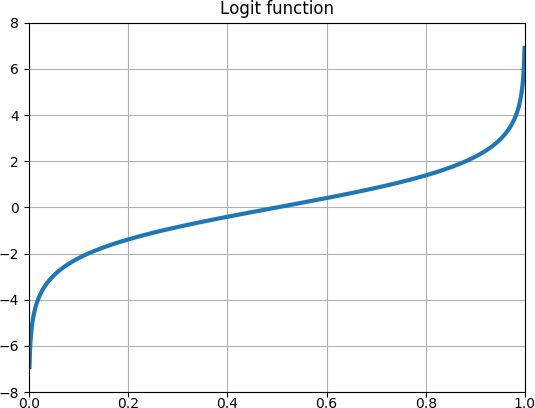
\includegraphics[clip, width=5cm]{../1/code/logit_func.png}
\end{center}
\end{minipage}
\end{tabular}
\end{center}
\end{figure}
この逆関数は,
\eqn{\text{logit}^{-1}(v)=\frac{e^v}{1+e^v}}
である.

$\because$
\eqn{v=\log \left(\frac{u}{1-u}\right),\ e^v=\frac{u}{1-u},\ e^v-ue^v=u,\ u=\frac{e^v}{1+e^v}}

\begin{itembox}[l]{\tcr{プロビット変換}}
…$(0,1)$から$(-\infty,\infty)$への変換$\Phi^{-1}(u)$(ただし, $\Phi$は標準正規累積分布関数)
\end{itembox}

…比率データを確率の形(0から1まで)に直し, $\Phi(u)$に当てはめてプロビット値を得ることをプロビット変換という.
これは標準正規分布のパーセント点を求めるのと同じである.

まず, 正規累積分布関数は
\eqn{\Phi(u)=\int_{-\infty}^u \text{N}(v|0,1)dv\ \text{ただし}\ \text{N}(v|0,1)=\tfrac{1}{\sqrt{2\pi}}\exp\left(-\tfrac{1}{2}v^2\right)}
である.
この逆関数が\tcr{プロビット関数}である.
プロビット関数は, 連続単調増加関数で,
\eqn{\Phi^{-1}(0)=-\infty,\ \Phi^{-1}(0.5)=0,\ \Phi^{-1}(1)=\infty}

\begin{figure}[H]
\begin{center}
\begin{tabular}{c}
% 1
\begin{minipage}{0.33\hsize}
\begin{center}
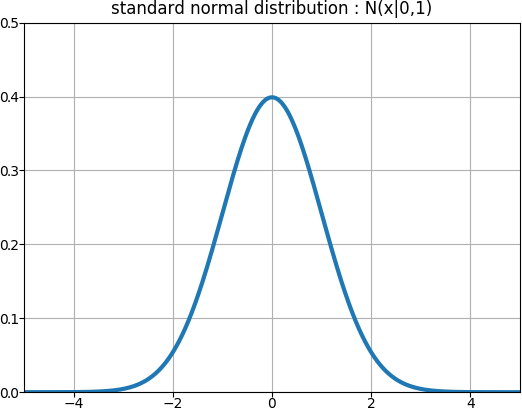
\includegraphics[clip, width=5cm]{../1/code/sn.png}
\end{center}
\end{minipage}
% 2
\begin{minipage}{0.33\hsize}
\begin{center}
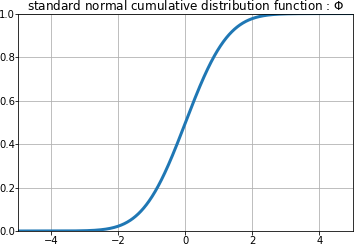
\includegraphics[clip, width=5cm]{../1/code/sn_cdf.png}
\end{center}
\end{minipage}
% 3
\begin{minipage}{0.33\hsize}
\begin{center}
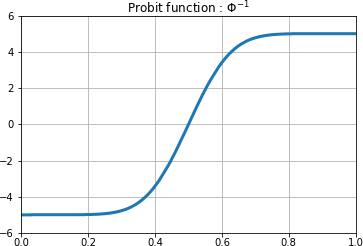
\includegraphics[clip, width=5cm]{../1/code/probit_func.png}
\end{center}
\end{minipage}
\end{tabular}
\end{center}
\end{figure}
ただし定義域の大部分で正の値にするため, 便宜上これに5を足してプロビット値とすることも多いらしい.

%==============================================================================================================%
\subsection{Computation and software}
\begin{itembox}[l]{ベイズデータ分析に含まれる計算タスク}
1.ベクトル操作と行列操作

2.確率密度関数の計算

3.確率分布からのシミュレーションの作成

4.構造化プログラミング

5.線形回帰推定と分散行列を計算する

6.1つのページに複数のグラフが表示する, 散布図を含むグラフィックス
\end{itembox}

…R, Stanなどがある.
Stanこの頃聞かないな...

\begin{itembox}[l]{累積分布関数}
\[F(v_*)=\text{Pr}(v\leq v_*)
=\begin{cases}
\sum_{v\leq v_*} p(v) &\text{if}\ p\ \text{is discreate}\\
\int_{-\infty}^{v_*} p(v)dv &\text{if}\ p\ \text{is continuous}
\end{cases}\]
\end{itembox}

…これを用いてサンプリングを行う手法, 逆cdf法がある.

例:$p(x)=\tfrac{3}{16}x^2$について試してみる.
\begin{figure}[H]
\begin{center}
\begin{tabular}{c}
% 1
\begin{minipage}{0.33\hsize}
\begin{center}
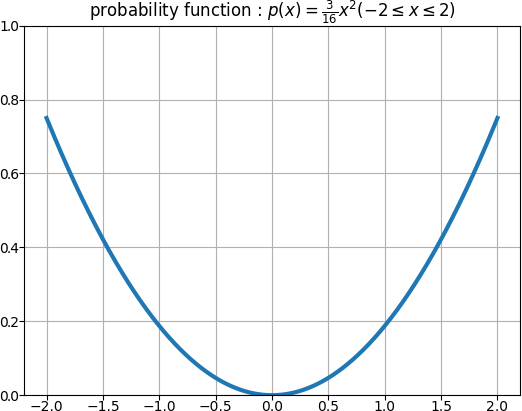
\includegraphics[clip, width=5cm]{../1/code/pf.png}
\end{center}
\end{minipage}
% 2
\begin{minipage}{0.33\hsize}
\begin{center}
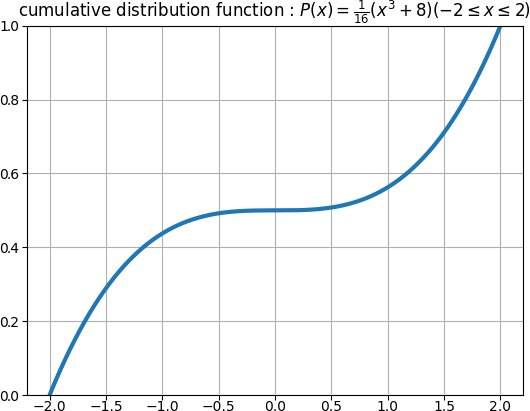
\includegraphics[clip, width=5cm]{../1/code/cdf.png}
\end{center}
\end{minipage}
% 3
\begin{minipage}{0.33\hsize}
\begin{center}
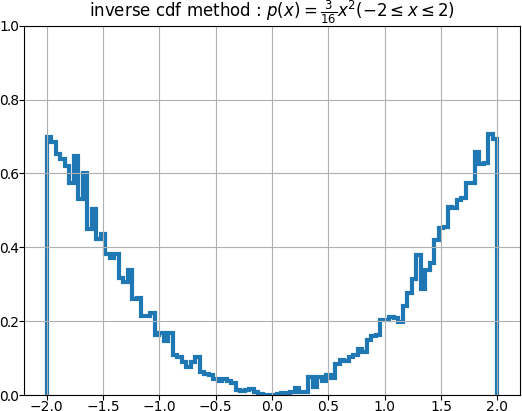
\includegraphics[clip, width=5cm]{../1/code/inverse_cdf.png}
\end{center}
\end{minipage}
\end{tabular}
\end{center}
\end{figure}
cdfの形が閉じた形で分かっている場合は結構使えるのでは?
ただ, argminの部分があるので結構計算量が大きい.


%==============================================================================================================%
\subsection{Bayesian inference in applied statistics}
\begin{itembox}[l]{ベイズ統計の主なテーマ}
1.多パラメータを使用する.

2.モデルの階層構造.

3.モデル検査.

4.単純な点推定ではなく, 分布の形での推論または少なくとも区間推定.

5.主要な計算方法としてのシミュレーションの使用.

6.ベイズモデルを明示的に呼び出すことができないデータ分析手法を理解し, 場合によっては改善するためのツールとしての確率モデルの使用.

7.モデル内のすべての変数に条件付きで, データがランダムサンプルとして表示されるという目標を近似するために, できるだけ多くの背景情報を分析に含めることの重要性.

8.興味のある推定量の推論がモデル過程に対してロバストになるように研究を設計することの重要性.
\end{itembox}

%==============================================================================================================%
\section{Single-parameter models}

\subsection{Estimating a probability from binomial data}
\begin{itembox}[l]{\tcr{ベルヌーイ試行}}
…成功か失敗がある確率で起こるような試行.
\eqn{p(y|\theta)=\theta^y(1-\theta)^{1-y}}
\end{itembox}

「例: コイントス」は通常, $\theta=\tfrac{1}{2}$で成功も失敗もともに確率$\tfrac{1}{2}$とする.


\begin{itembox}[l]{\tcr{二項モデル}}
…ベルヌーイ試行の系列, 二項分布に従うモデル.
\eqn{p(y|\theta)=\text{Bin}(y|n,\theta)=\left(\begin{array}{c}n\\y\end{array}\right)\theta^y(1-\theta)^{n-y}}
\end{itembox}

あるベルヌーイ分布に従う試行を$n$回繰り返したもので, ある成功の回数に対する確率を考えるモデル.
\begin{figure}[H]
\begin{center}
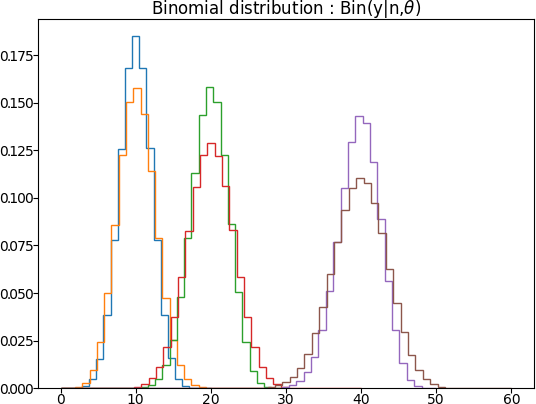
\includegraphics[clip, width=5cm]{../2/code/Binomial.png}
\end{center}
\end{figure}

\begin{itembox}[l]{二項分布の事前分布}
1.Laplaceは一様事前分布を用いた.

2.共役事前分布はベータ分布である.
\end{itembox}

Laplaceが一様分布を事前分布に用いたのは, \tcr{不十分な理由の原則}(2.4節)に基づくもので, なんもわからんから一様に確率を割り当てようという考えからである.
\eqn{\text{U}(\theta|0,1)=1,\ 0\leq \theta\leq 1}

また, 一般的に共役分布であるベータ分布を用いて解析を行うことが多い.
ベータ分布
\eqn{\text{Beta}(\theta|\alpha,\beta)=\frac{\Gamma(\alpha+\beta)}{\Gamma(\alpha)\Gamma(\beta)}\theta^{\alpha-1} (1-\theta)^{\beta-1}}
\begin{figure}[H]
\begin{center}
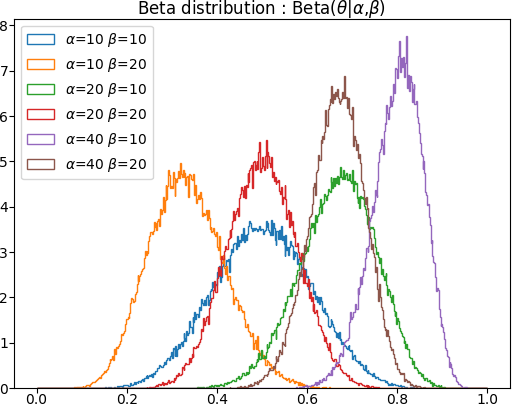
\includegraphics[clip, width=5cm]{../2/code/Beta.png}
\end{center}
\end{figure}


\begin{itembox}[l]{\tcr{ラプラスの連続法則}}
…一様事前分布を用いた二項モデルの事後予測分布についての式のこと.
\end{itembox}
$\because$
パラメータ$\theta$は成功率なので, $0\leq \theta \leq 1$の範囲にある.
そこで, 二項モデルの事前分布として, $[0,1]$上の一様分布を用いた場合について考える.
事前分布を
\eqn{\text{U}(\theta|0,1)=1,\ 0\leq \theta\leq 1}
のように設定するのである.
そのとき, 尤度関数は
\eqn{p(y|\theta)=\text{Bin}(y|n,\theta)=\left(\begin{array}{c}n\\y\end{array}\right)\theta^y(1-\theta)^{n-y}}
であるので,
\eqn{\text{Pr}(\theta\in(\theta_1,\theta_2)|y)
&=\frac{\text{Pr}(\theta\in(\theta_1,\theta_2),y)}{p(y)}=\frac{\int_{\theta_1}^{\theta_2}p(y|\theta)p(\theta)d\theta}{p(y)}\\
&=\frac{\int_{\theta_1}^{\theta_2}\left(\begin{array}{c}n\\y\end{array}\right)\theta^y(1-\theta)^{n-y}}{p(y)}d\theta}
となる.
また, 分母は
\eqn{p(y)
&=\int_0^1 p(y|\theta)d\theta=\int_0^1\left(\begin{array}{c}n\\y\end{array}\right)\theta^y(1-\theta)^{n-y}d\theta=\left(\begin{array}{c}n\\y\end{array}\right) \int_0^1 \theta^y (1-\theta)^{n-y}d\theta\\
&=\left(\begin{array}{c}n\\y\end{array}\right) \left( \frac{1}{y+1}\left[\theta^{y+1}(1-\theta)^{n-y}\right]_0^1+\frac{n-y}{y+1} \int_0^1\theta^{y+1}(1-\theta)^{n-y+1}d\theta\right)\\
&=\left(\begin{array}{c}n\\y\end{array}\right) \frac{n-y}{y+1} \left(\begin{array}{c}n\\y+1\end{array}\right)^{-1} p(y+1)\\
&=p(y+1)}
これより,
\eqn{p(y)=\frac{1}{n+1},\ \text{for}\ n=0,\dots,n}
従って,
\eqn{\text{Pr}(\theta\in(\theta_1,\theta_2)|y)
=(n+1)\int_{\theta_1}^{\theta_2}\left(\begin{array}{c}n\\y\end{array}\right)\theta^y(1-\theta)^{n-y}d\theta}
である.

また事後予測分布は
\eqn{\text{Pr}(\tilde{y}=1|y)&=\int_0^1 \text{Pr}(\tilde{y}=1|\theta,y)p(\theta|y)d\theta=\int_0^1 \theta p(\theta|y)d\theta\\
&=\int_0^1(n+1) \left(\begin{array}{c}n\\y\end{array}\right)\theta^{y+1}(1-\theta)^{n-y}d\theta=(n+1)\left(\begin{array}{c}n\\y\end{array}\right)\left(\begin{array}{c}n+1\\y+1\end{array}\right)^{-1} \frac{1}{n+2}\\
&=\frac{y+1}{n+2}}
ここで, $y=0$と$y=n$場合について考える場合.
\eqn{\text{Pr}(\tilde{y}=1|y=0)=\frac{1}{n+2},\ \text{Pr}(\tilde{y}=1|y=n)=\frac{n+1}{n+2}}
この結果は, 一様事前分布に基づいた, 「ラプラスの連続法則」として知られている.


%==============================================================================================================%
\subsection{Posterior as compromise between data and prior information}
\begin{itembox}[l]{事後分布は事前分布と尤度の妥協点}
…事後分布は事前情報とデータの間の妥協点と表される点に集中し, サンプルサイズが大きくなるつれて, データによって妥協がより大きく支配される.
\end{itembox}

ベイズ統計とは, 事前分布と尤度関数の明示的な指定がカギである.
$n\rightarrow \infty$において, 尤度が事前分布を支配してしまうということは, ほぼ頻度主義に近づいていくということを意味するのではないだろうか?
つまり, 漸近理論($n\rightarrow \infty$)とベイズ統計は相性がいいように思えない.
少サンプルでこそベイズ統計の真価が発揮できるのではないだろうか.
また, 事前分布を尤度関数のブレーキ役であると考えるならば, 外れ値を含むような少サンプルにおいて強い理論になりうるだろう.
そうでなければ, 頻度主義の統計とさほど変わらない.

%==============================================================================================================%
\subsection{Summarizing posterior inference}
\begin{itembox}[l]{シミュレーションによって実装されるベイズ手法のメリット}
…複雑な変換の後でさえ, 事後推論を要約することができる柔軟性である.
\end{itembox}

モンテカルロシミュレーションとか.


\begin{itembox}[l]{位置についての要約}
…分布の平均, 中央値, モード
\end{itembox}

それぞれ, 位置についての要約統計量である.


\begin{itembox}[l]{分散についての要約}
…標準偏差, 四分位範囲, 他の分位数
\end{itembox}

それぞれスケールについての要約統計量である.
\tcr{四分位範囲(interquartile range)}はあんまり, 初等統計の本で見ない.

第2四分位数は中央値である.
第1, 第3四分位数の差を四分位範囲と呼ぶ.
これは, ロバストなスケール統計量であることも知られている.
\begin{figure}[H]
\begin{center}
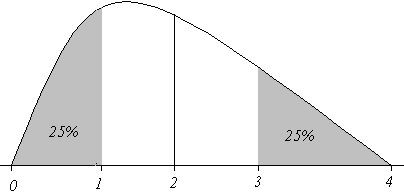
\includegraphics[clip, width=8cm]{../2/code/quantile.jpg}
\end{center}
\end{figure}

分位数(quantile)は25\%区切れでないものを指す.

\begin{itembox}[l]{区間推定量}
…事後分布において質量が$100(1-\alpha)\%$存在する中心の区間などをいう.
\end{itembox}

分位数を用いる.


%==============================================================================================================%
\subsection{Informative prior distributions}
\begin{itembox}[l]{\tcr{不十分な理由の原則}}
…Laplaceが二項モデルの事前分布として, 一様分布を用いたように, 何も知らない場合は一様分布を用いるべきであるという主張.
\end{itembox}

なんもわからんから一様に確率を割り当てようという考えからである.
\eqn{\text{U}(\theta|0,1)=1,\ 0\leq \theta\leq 1}


\begin{itembox}[l]{\tcr{超パラメータ}}
…事前分布のパラメータのこと.
\end{itembox}


\begin{itembox}[l]{\tcr{共役}}
…事後分布が事前分布と同じパラメトリック形式に従うという性質をいう.
その分布族のことを\tcr{共役分布族}という.
\end{itembox}

次の, 例を見れば分かる.


\begin{itembox}[l]{二項分布の共役事前分布}
…Beta$(\alpha,\beta)$で, 超パラメータは$\alpha$回の成功, $\beta$回の失敗と考えられる.
\end{itembox}
共役事前分布であるベータ分布を用いた解析について考える.

$\because$
二項モデルでは上で示したように, 尤度関数は
\eqn{p(y|\theta)=\text{Bin}(y|n,\theta)=\left(\begin{array}{c}n\\y\end{array}\right)\theta^y(1-\theta)^{n-y}}
であるので, 共役分布族は
\eqn{p(y|\theta)\propto \theta^a (1-\theta)^b}
という形をとる分布である.
これより, 事前分布を
\eqn{p(\theta)\propto \theta^{\alpha-1} (1-\theta)^{\beta-1}}
となるように選べば\tcr{共役性}が成り立つ.
ここで, ベータ分布
\eqn{\text{Beta}(\theta|\alpha,\beta)=\frac{\Gamma(\alpha+\beta)}{\Gamma(\alpha)\Gamma(\beta)}\theta^{\alpha-1} (1-\theta)^{\beta-1}}
を選ぶ.
すると, ベイズ則のコア「事後分布$\propto$事前分布$\times$尤度関数」より,
\eqn{p(\theta|y)
&\propto p(\theta)p(y|\theta)\\
&\propto \theta^y (1-\theta)^{n-y} \theta^{\alpha-1} (1-\theta)^{\beta-1}\\
&=\theta^{y+\alpha-1} (1-\theta)^{n-y+\beta-1}\\
&=\text{Beta}(\theta|\alpha+y,\beta+n-y)}
となる.

データにおいて, $y$回成功, $n-y$回失敗であり, 事後$\alpha+y$回成功, $\beta+n-y$回失敗と考えることが分かるので.
事前分布, Beta($\alpha,\beta$)は, 事前に$\alpha$回成功, $\beta$回失敗という意味があると考えられる.


\begin{itembox}[l]{\tcr{非共役事前分布}}
…事後推論の解釈を不透明にし, 計算を困難にすることがあるが, 概念的に問題はない.
複雑なモデルの場合は使えない.
\end{itembox}

共役分布を用いるメリットは, 事前分布と事後分布のパラメトリック形式が一致するという概念的理由と, 解析上の簡易性というのが主な理由である.
この点において, 非共役事前分布を用いることはダメではない.
ただその使用にあたっては, しっかりとした理由がある必要がある.


\begin{itembox}[l]{\tcr{指数型分布族}}
\[p(y_i|\theta)=f(y_i)g(\theta)e^{\phi(\theta)^{\mathrm{T}}u(y_i)}\]
\end{itembox}

ベータ, ガンマ, フォンミューゼス分布などほかにも多くの分布が指数型分布族に属する.

ベータ分布
\eqn{\text{Beta}(\theta|\alpha,\beta)=\frac{\Gamma(\alpha+\beta)}{\Gamma(\alpha)\Gamma(\beta)}\theta^{\alpha-1}(1-\theta)^{\beta-1}}
に対しては,
\eqn{f(\theta)=1,\ g(\alpha,\beta)=\frac{\Gamma(\alpha+\beta)}{\Gamma(\alpha)\Gamma(\beta)},\ \phi(\alpha,\beta)=\left(\begin{array}{c}\alpha-1\\\beta-1\end{array}\right),\ u(\theta)=\left(\begin{array}{c}\ln\theta\\\ln(1-\theta)\end{array}\right)}
他についてはPRML演習2.56参照.


%==============================================================================================================%
\subsection{Estimating a normal mean with known variance}
\begin{itembox}[l]{\tcr{正規モデル}(単一観測に対する, ただし, 平均未知, 分散既知)}
\[p(y|\theta)=\frac{1}{\sqrt{2\pi}\sigma}e^{-\frac{1}{2\sigma^2}(y-\theta)^2}(=\text{N}(y|\theta,\sigma^2))\]
\end{itembox}


\begin{itembox}[l]{正規モデルの平均$\theta$に対する共役事前分布}
…正規分布N$(\mu_0,\sigma_0^2)$は共役事前分布である.
また, 事後分布は正規分布となる.
\eqn{p(\theta|y)=\text{N}(\mu_1,\tau^2_1),\ \mu_1=\tfrac{1/\tau_0^2 \mu_0+1/\sigma^2 y}{1/\tau_0^2+1/\sigma^2}\ \text{and}\  \tfrac{1}{\tau_1^2}=\tfrac{1}{\tau_0^2}+\tfrac{1}{\sigma^2}}
\end{itembox}
$\because$
まず, 共役事前分布の導出であるが,
\eqn{p(y|\theta)=\frac{1}{\sqrt{2\pi}\sigma}e^{-\frac{1}{2\sigma^2}(y-\theta)^2}(=\text{N}(y|\theta,\sigma^2))\propto\exp\left(-\frac{1}{2\sigma^2}(y-\theta)^2\right)}
より, 正規分布が共役事前分布であることが分かる.
事後分布については以下(n個の観測値に対する一般化)参照.


\begin{itembox}[l]{事後平均についての解釈}
…事後平均は事前精度とデータ精度を重みとする, 事前平均とデータ平均の重み付き平均である.
\end{itembox}

これも以下参照.


\begin{itembox}[l]{事後予測分布}
\[p(\tilde{y}|y)=\text{N}(\tilde{y}|\mu_1,\sigma^2+\tau^2_1)\]
と直接積分から求めることができ, 平均は同じであるが分散は大きくなる.
\end{itembox}
$\because$
積分計算を行う
\eqn{p(\tilde{y}|y)
&=\int p(\tilde{y}|\theta)p(\theta|y) d\theta\\
&=\int \frac{1}{\sqrt{2\pi\sigma^2}}\exp \left(-\tfrac{1}{2\sigma^2}(\tilde{y}-\theta)^2\right)\frac{1}{\sqrt{2\pi\tau_1^2}} \exp \left(-\tfrac{1}{2\tau_1^2}(\theta-\mu_1)^2\right)d\theta\\
&= \frac{1}{\sqrt{2\pi\sigma^2}\sqrt{2\pi\tau_1^2}}\int \exp \left(-\tfrac{1}{2} \left( \left( \tfrac{1}{\sigma^2}+\tfrac{1}{\tau_1^2}\right)\theta^2-2\left(\tfrac{1}{\sigma^2}\tilde{y}+\tfrac{1}{\tau_1^2}\mu_1\right)\theta+\left(\tfrac{1}{\sigma^2}\tilde{y}^2+\tfrac{1}{\tau_1^2}\mu_1^2\right)\right)\right)d\theta\\
&= \frac{1}{\sqrt{2\pi\sigma^2}\sqrt{2\pi\tau_1^2}}\int \exp \left(-\tfrac{1}{2} \left(a\theta^2-2b\theta+c\right)\right)d\theta\\
&= \frac{1}{\sqrt{2\pi\sigma^2}\sqrt{2\pi\tau_1^2}}\exp\left(-\tfrac{1}{2}\left(c-\tfrac{b^2}{a}\right)\right) \int \exp \left(-\tfrac{1}{2a^{-1}}\left(\theta-\tfrac{b}{a}\right)^2 \right)d\theta\\
&= \frac{1}{\sqrt{2\pi\sigma^2}\sqrt{2\pi\tau_1^2}}\exp\left(-\tfrac{1}{2}\left(c-\tfrac{b^2}{a}\right)\right) \sqrt{2\pi a^{-1}}\\
&= \frac{1}{\sqrt{2\pi\sigma^2}\sqrt{2\pi\tau_1^2}}\exp\left(-\tfrac{1}{2}\left(c-\tfrac{b^2}{a}\right)\right) \sqrt{2\pi \tfrac{\sigma^2\tau_1^2}{\sigma^2+\tau_1^2}}\\
&= \frac{1}{\sqrt{2\pi(\sigma^2+\tau_1^2)}}\exp\left(-\tfrac{1}{2(\sigma^2+\tau_1^2)}\left(\tilde{y}-\mu_1\right)\right)}





\begin{itembox}[l]{正規モデル(複数観測に対する, ただし, 平均未知, 分散既知)}
…iddに従う観測値$y=(y_1,\dots,y_n)$についても考えるが, ほとんどアナロジーと一致する.
$\bar{y}$が十分統計量であるので, $\bar{y}|\theta, \sigma^2 \sim \text{N}(\theta,\sigma^2/n)$なので, 単一正規観測値で導かれる結果は適用すれば, 
\eqn{p(\theta|y_1,\dots,y_n)=p(\theta|\bar{y})=\text{N}(\theta|\mu_n,\tau_n^2),\ \mu_n=\tfrac{1/\tau_0^2 \mu_0+n/\sigma^2\bar{y}}{1/\tau_0^2+n/\sigma^2}\ \text{and}\  \tfrac{1}{\tau_n^2}=\tfrac{1}{\tau_0^2}+\tfrac{n}{\sigma^2}}
を得られる.
\end{itembox}
$\because$
事後分布は
\eqn{p(\theta|y)&\propto p(\theta)p(y|\theta)=p(\theta)\prod_{i=1}^n p(y_i|\theta)\propto \exp\left(-\tfrac{1}{2\tau_0^2}(\theta-\mu_0)^2\right) \prod_{i=1}^n \exp\left(-\tfrac{1}{2\sigma^2}(y_i-\theta)^2\right)\\
&\propto \exp\left(-\tfrac{1}{2}  \left( \tfrac{1}{\tau_0^2}(\theta-\mu_0)^2+\tfrac{1}{\sigma^2}\sum_{i=1}^n (y_i-\theta)^2\right)\right)\\
&=\exp\left(-\frac{1}{2}\left( \left(\tfrac{1}{\tau_0^2}+\tfrac{n}{\sigma^2}\right) \theta^2-2\left(\tfrac{1}{\tau_0^2}\mu_0+\tfrac{1}{\sigma^2}\sum_{i=1}^n y_i\right)\theta + \cdots \right) \right)\\
&=\exp\left(-\frac{1}{2}\left(\tfrac{1}{\tau_0^2}+\tfrac{n}{\sigma^2}\right) \left(\theta^2-2\left(\tfrac{1}{\tau_0^2}+\tfrac{n}{\sigma^2}\right)^{-1}\left(\tfrac{1}{\tau_0^2}\mu_0+\tfrac{n}{\sigma^2}\bar{y}\right)\theta + \cdots \right) \right)\\
&\propto\exp\left(-\frac{1}{2}\left(\tfrac{1}{\tau_0^2}+\tfrac{n}{\sigma^2}\right) \left(\theta-\left(\tfrac{1}{\tau_0^2}+\tfrac{n}{\sigma^2}\right)^{-1}\left(\tfrac{1}{\tau_0^2}\mu_0+\tfrac{n}{\sigma^2}\bar{y}\right)\right)^2 \right)}
これより, 事後分布は事後平均, 事後分散は
\eqn{\mu_n=\tfrac{1/\tau_0^2 \mu_0+n/\sigma^2\bar{y}}{1/\tau_0^2+n/\sigma^2}\ \text{and}\  \tfrac{1}{\tau_n^2}=\tfrac{1}{\tau_0^2}+\tfrac{n}{\sigma^2}}
となるような正規分布
\eqn{p(\theta|y_1,\dots,y_n)=\text{N}(\theta|\mu_n,\tau_n^2)}
となる.
 

\begin{itembox}[l]{事後平均についての解釈}
…$n$が大きくなるにしたがって, データ精度の重みが大きくなることが分かる.
また, 分散は小さくなっていく.
\end{itembox}

$\because$
事後平均については$n\rightarrow \infty$において, $\mu_n\rightarrow \bar{y}$になり, $\tau_n^2\rightarrow 0$である.

\begin{itembox}[l]{事後予測分布}
…分散が小さくなっていき, より良い予測が可能になるという点で, 感覚と一致する
\end{itembox}

ただ,
\eq{p(\tilde{y}|y)=\text{N}(\tilde{y}|\mu_n,\sigma^2+\tau^2_n)}
ということで, 完全に予測することは不可能であるということが分かる.


%==============================================================================================================%
\subsection{Other standard single-parameter models}
\begin{itembox}[l]{\tcr{二項分布}}
…交換可能な結果を数えるとき用いられる.
\end{itembox}


\begin{itembox}[l]{\tcr{正規分布}}
…交換可能な独立項の和である確率変数に適用される.
また, 正のデータの対数に正規分布を適用する機会がある.
\end{itembox}


\begin{itembox}[l]{\tcr{ポアソン分布}, \tcr{指数分布}}
…すべての時間間隔で交換可能に発生するとモデル化されたイベントのカウント数および待ち時間としてそれぞれ発生します.
\end{itembox}


\begin{itembox}[l]{正規モデル(ただし, 平均既知, 分散未知)}
…十分統計量はサンプル分散で, 共役事前分布は\tcr{逆-ガンマ分布}である.
\eqn{v=\frac{1}{n}\sum_{i=1}^n(y_i-\theta)^2,\ p(\sigma^2)\propto (\sigma^2)^{-(\alpha+1)}e^{-\beta/\sigma^2}}
便利なパラメータ化\tcr{逆-$\chi^2$分布}を用いると, 事前分布, 事後分布は
\eqn{\sigma^2\sim \text{Inv-}\chi^2(\nu_0,\sigma_0^2),\ \sigma^2|y\sim \text{Inv-}\chi^2\left(\nu_0+n,\tfrac{\nu_0\sigma_0^2+nv}{\nu_0+n}\right)}
\end{itembox}
$\because$
尤度関数が,
\eqn{p(y|\sigma^2)&\propto \sigma^{-n}\exp\left(-\frac{1}{2\sigma^2}\sum_{i=1}^n(y_i-\theta)^2\right)\\
&=(\sigma^2)^{-n/2}\exp \left(-\frac{n}{2\sigma^2}v\right)}
ただし, $v$は十分統計量で
\eqn{v=\frac{1}{n}\sum_{i=1}^n(y_i-\theta)^2}
である.
また, このことから, 
\eqn{p(\sigma^2)\propto (\sigma^2)^{-(\alpha+1)}e^{-\beta/\sigma^2}}
というパラメトリック形式の共役事前分布を探す.
\tcr{ガンマ分布}は
\eqn{\text{Gamma}(x|k,\theta)=x^{k-1}\frac{e^{-x/\theta}}{\Gamma(k)\theta^k}}
\begin{figure}[H]
\begin{center}
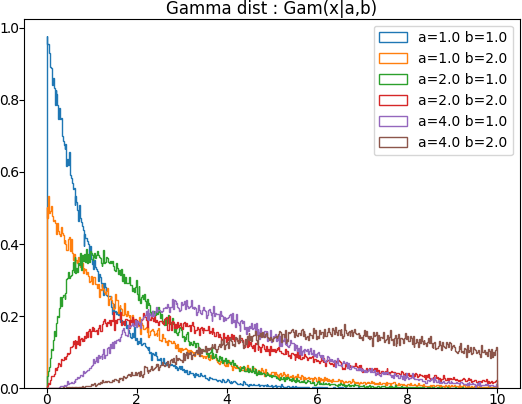
\includegraphics[clip, width=5cm]{../2/code/Gamma.png}
\end{center}
\end{figure}
であるが, \tcr{逆-ガンマ分布}は変数変換の公式より
\eqn{\text{Inv-Gamma}(x|k,\theta)
&=\text{Gamma}\left(\tfrac{1}{x}|k,\theta\right)/x^2\\
&=x^{-k-1}\frac{e^{-1/x\theta}}{\Gamma(k)\theta^k}}
これより, 共役事前分布として, 逆-ガンマ分布を選ぶことにする.
\eqn{\text{Inv-Gamma}(\sigma^2|\alpha,\beta)=\frac{1}{\Gamma(\alpha)} \beta^{\alpha} (\sigma^2)^{-(\alpha+1)} \exp\left(-\beta/\sigma^2 \right)}
ここで, 逆-$\chi^2$分布
\eqn{\text{Inv-}\chi^2(\theta|v,s^2)=\frac{\left(\tfrac{v}{2}\right)^{\tfrac{v}{2}}}{\Gamma\left(\tfrac{v}{2}\right)}s^v\theta^{-\left(\tfrac{v}{2}+1\right)}\exp\left(-\tfrac{vs^2}{2\theta}\right)}
は
\eqn{\text{Inv-Gamma}(\sigma^2|\alpha=\tfrac{v}{2},\beta=\tfrac{v}{2}s^2)&
=\frac{1}{\Gamma(\tfrac{v}{2})} (\tfrac{v}{2}s^2)^{\tfrac{v}{2}} (\sigma^2)^{-(\tfrac{v}{2}+1)} \exp\left(-(\tfrac{v}{2} s^2)/\sigma^2 \right)=\text{Inv-}\chi^2(\sigma^2|v,s^2)}
より, Inv-Gamma$\left(\theta|\alpha=\tfrac{v}{2},\beta=\tfrac{v}{2}s^2\right)$と一致する.

(\url{http://miyahn.blog80.fc2.com/blog-entry-116.html}参照)

このパラメータ変換は1対1であるので, どっちを使っても同じ.
このパラメータ化の方が便利らしく, ここでは後者を用いる.

事後分布の計算は,
\eqn{p(\sigma^2|y)
&\propto p(\sigma^2)p(y|\sigma^2)=\text{Inv-Gamma}(\sigma^2|\nu_0,\sigma_0^2)\text{N}(y|\sigma^2)\\
&\propto \left(\frac{\sigma_0^2}{\sigma^2}\right)^{\nu_0/2+1} \exp\left(-\frac{\nu_0\sigma_0^2}{2\sigma^2}\right)\cdot (\sigma^2)^{-n/2}\exp \left(-\frac{n}{2}\frac{v}{\sigma^2}\right)\\
&\propto (\sigma^2)^{-((n+\nu_0)/2+1)} \exp\left(-\frac{1}{2\sigma^2} (\nu_0\sigma_0^2+nv)\right)}
となる.
従って,
\eqn{\sigma^2|y\sim \text{Inv-}\chi^2\left(\nu_0+n,\frac{\nu_0\sigma_0^2+nv}{\nu_0+n}\right)}

ここでは, 分散の事前分布として逆-ガンマ分布を用いたが, 精度の事前分布としてガンマ分布を用いてもよい.

\begin{itembox}[l]{\tcr{ポアソンモデル}(ただし, 割合未知)}
…割合$\theta$のポアソン分布に従うなら, 単一観測値$y$の確率分布は
\eqn{p(y|\theta)=\frac{\theta^ye^{-\theta}}{y!},\ \text{for}\ y=0,1,\cdots}
で, 独立同一分布に従う観測値のベクトル$y=(y_1,\cdots,y_n)$の尤度は,
\eqn{p(y|\theta)=\prod_{i=1}^n\frac{1}{y_i!}\theta^{y_i}e^{-\theta}}
共役事前分布は\tcr{ガンマ分布}, Gamma$(\alpha,\beta)$で事後分布は
\eqn{\theta|y\sim \text{Gamma}(\alpha+n\bar{y},\beta+n)}
単一観測値$y$のポアソンモデルの事前予測分布は\tcr{負の二項分布}
\eqn{p(y)&=\tfrac{p(y|\theta)p(\theta)}{p(\theta|y)}=\tfrac{\text{Poisson}(y|\theta)\text{Gamma}(\theta|\alpha,\beta)}{\text{Gamma}(\theta|\alpha+y,1+\beta)}=\tfrac{\Gamma(\alpha+y)\beta^{\alpha}}{\Gamma(\alpha)y!(1+\beta)^{\alpha+y}}\\
&=\left(\begin{array}{c}\alpha+y-1\\y\end{array}\right) \left(\frac{\beta}{\beta+1}\right)^{\alpha}\left(\frac{1}{\beta+1}\right)^y=\text{Neg-bin}(\alpha,\beta)}
\end{itembox}

$\because$
まず,
\eqn{p(y|\theta)=\prod_{i=1}^n\frac{1}{y_i!}\theta^{y_i}e^{-\theta}\propto\theta^{\sum y_i} e^{-n\theta}}
より,
\eqn{\text{Gamma}(\theta|\alpha,\beta)=\theta^{\alpha-1}\beta^{\alpha}\frac{e^{-\beta\theta}}{\Gamma(\alpha)}}
は共役事前分布であることが分かる.
事後分布は,
\eqn{p(\theta|y)
&\propto p(\theta)p(y|\theta)\\
&\propto \theta^{\alpha-1}\beta^{\alpha}\frac{e^{-\beta\theta}}{\Gamma(\alpha)}\theta^{\sum y_i} e^{-n\theta}\propto \theta^{\alpha-1}e^{\beta\theta}\theta^{\sum y_i} e^{-n\theta}\\
&=\theta^{\alpha+n\bar{y}-1}e^{(\beta+n)\theta}}
これより,
\eqn{\theta|y\sim \text{Gamma}(\alpha+n\bar{y},\beta+n)}
となる.



\begin{itembox}[l]{ポアソンモデル(割合と暴露のモデル)}
…データ点$y_1,\dots,y_n$に対して,
\eqn{y_i\sim \text{Poisson}(x_i\theta)}
とするモデルがある.
$x_i$は暴露で$\theta$は割合である.
$\theta$に対する共役事前分布はガンマ分布であり, ともに事後分布は
\eqn{\theta\sim\text{Gamma}(\alpha,\beta),\ \theta|y \sim \text{Gamma}\left(\alpha+\sum_{i=1}^n y_i, \beta+\sum_{i=1}^n x_i\right)}
\end{itembox}
このモデルは全体で$x_i$回の中で, 割合$\theta$で満たす事象の起こる回数$y_i$を考えるというもの.

$\because$
上と同じ事前分布(ガンマ分布)が共役であることは明らかであるが, 事後分布を考えたとき,
\eqn{p(\theta|y)
&\propto \theta^{\alpha-1}\beta^{\alpha}\frac{e^{-\beta\theta}}{\Gamma(\alpha)} \prod_{i=1}^n\frac{1}{y_i!}(x_i\theta)^{y_i}e^{-x_i\theta} \\
&\propto \theta^{\alpha-1}e^{-\beta\theta} \theta^{\sum y_i} e^{-\sum x_i\theta} \\
&\propto \theta^{\alpha+\sum y_i-1} e^{-(\beta+\sum x_i)\theta}}
より,
\eqn{p(\theta|y)=\text{Gamma}\left(\theta \left|\alpha+\sum_{i=1}^n y_i-1,\beta+\sum_{i=1}^n x_i\right.\right)}


\begin{itembox}[l]{\tcr{指数モデル}}
…一般的に待ち時間モデルやしばしば時間スケールの連続で正の実数値確率変数などに使われる.
パラメータ$\theta$が与えられた, 結果$y$のサンプリング分布は
\eqn{p(y|\theta)=\theta\exp(-y\theta),\ \text{for}\ y>0}
\tcr{無記憶性}をもつ.
任意の$s, t$に対し$\text{Pr}(y>t+s|y>s,\theta)=\text{Pr}(y>t|\theta)$.
ポアソン分布と同じく, 共役事前分布は$\text{Gamma}(\theta|\alpha,\beta)$で, 対応する事後分布は$\text{Gamma}(\theta|\alpha+1,\beta+y)$である.
\end{itembox}
$\because$
指数分布が
\eqn{p(y|\theta)=\theta\exp(-y\theta),\ \text{for}\ y>0}
であるため, ガンマ分布
\eqn{\text{Gamma}(\theta|\alpha,\beta)=\theta^{\alpha-1}\beta^{\alpha}\frac{e^{-\beta\theta}}{\Gamma(\alpha)}}
は共役事前分布として使える.
事後分布は
\eqn{p(\theta|y)
&\propto  \theta^{\alpha-1}e^{-\beta\theta} \theta e^{(-y\theta)}\\
&= \theta^{\alpha+1-1} e^{-(\beta+y)\theta}}
より,
\eqn{p(\theta|y)=\text{Gamma}(\theta|\alpha+1,\beta+y)}
となる.


%==============================================================================================================%
\subsection{Example: informative prior distribution for cancer rates}


%==============================================================================================================%
\subsection{Noninformative prior distributions}
\begin{itembox}[l]{\tcr{参照事前分布}}
…事前分布に母集団の基礎がない場合は, 構築が困難であり, 事後分布において最小限の役割を果たすことが保証され得る事前分布が望まれてきた.
「データが, 自分自身について話すようにする」
\end{itembox}

共役事前分布を用いるということは, 事後分布ンパラメータ形式を制限するということにつながる.
それが望ましくない場合, 非共役なものを用いることで, 尤度関数に重きを置いた事後分布を構築することができる.


\begin{itembox}[l]{\tcr{弱情報事前分布}}
…事後分布を\tcr{正規化}するのに十分な情報を含むもの.
\end{itembox}


\begin{itembox}[l]{\tcr{適切}, \tcr{不適切}}
…積分して1になる, または発散するような分布関数のこと.
\end{itembox}

不適切な確率分布を用いていいということに結構驚く.


\begin{itembox}[l]{\tcr{非正規化密度}}
…積分値が正の有限値になる分布関数のこと.
\end{itembox}

正規加項をかければ済むが, それが分からないときに用いる.


\begin{itembox}[l]{正規モデル(ただし, 平均既知, 分散未知)}
…無情報事前分布を, 逆-$\chi^2$分布とすると, 事後分布は
\eqn{p(\sigma^2|y)\approx \text{Inv-}\chi^2(\sigma^2|n,v)}
この式は, 事前密度を$p(\sigma^2)\propto 1/\sigma^2$とすることでも導けるが, これは不適切な事前分布である.
\end{itembox}
$\because$
まず, $p(\sigma^2)=1/\sigma^2$が不適切な分布であることはすぐにわかる.
また, これを事前分布として用いた正規モデルを考える.
\eqn{p(\sigma^2|y)
&\propto p(\sigma^2)p(y|\sigma^2)\\
&\propto \tfrac{1}{\sigma^2}\sigma^{-n}\exp\left(-\frac{n}{2\sigma^2}v\right)
=\sigma^{\tfrac{n}{2}-2}\exp\left(-\frac{n}{2\sigma^2}v\right)\\
&\propto\text{Inv-}\chi^2(\sigma^2|n,v)}
となる.


\begin{itembox}[l]{\tcr{Jeffreysの不変原理}}
…無情報事前密度を$p(\theta)\propto[J(\theta)]^{1/2}$として定義する.
ここで, $J(\theta)$は$\theta$の\tcr{フィッシャー情報}である.
\eqn{J(\theta)=\text{E}\left(\left(\left. \tfrac{d\log p(y|\theta)}{d\theta}\right)^2\right|\theta\right)=\text{E}\left(\left.\tfrac{d^2\log p(y|\theta)}{d\theta^2}\right|\theta\right)}
\end{itembox}


\begin{itembox}[l]{二項パラメータに対する無情報事前分布}
…Jeffreys事前分布は$p(\theta)\propto\theta^{-1/2}(1-\theta)^{-1/2}$で, $\text{Beta}(\tfrac{1}{2},\tfrac{1}{2})$密度である.

ベイズ-ラプラス一様事前密度は$\theta\sim\text{Beta}(1,1)$で表せる.

指数関数表現の自然パラメータで一様事前密度は$p(\text{logit}(\theta))\propto\text{constant}$である.
不適切な$\text{Beta}(0,0)$に対応する.
\end{itembox}
△
$\because$
Jeffreys事前分布は
\eqn{\tfrac{d^2\log p(y|\theta)}{d\theta^2}
&=\tfrac{d^2}{d\theta^2}\text{Bin}(y|n,\theta)=\tfrac{d^2}{d\theta^2}\left(\begin{array}{c}n\\y\end{array}\right)\theta^y(1-\theta)^{n-y}\\
&=\theta^{-2} y(y-1) \text{Bin}(y|n,\theta) - \theta^{-1}(1-\theta)^{-1} y(n-y) \text{Bin}(y|n,\theta) + (1-\theta)^{-2} (n-y)(n-y-1) \text{Bin}(y|n,\theta)}
より,
\eqn{J(\theta)
&\propto \theta^{-2}(n\theta(1-\theta)-n\theta) - \theta^{-1}(1-\theta)^{-1}(n^2\theta-n\theta(1-\theta)) +  (1-\theta)^{-2}(n^2-2n^2\theta+n\theta(1-\theta)-n+n\theta)\\
&=-\theta^{-2}(n\theta^2) - (1-\theta)^{-1}(n^2-n+n\theta) +n(n-1)(1-2\theta)(1-\theta)^{-2} - n\theta^2(1-\theta)^{-2}\\
&\ \vdots\\
&\propto \theta^{-1}(1-\theta)^{-1}}
ということを示せればよいが...


ベイズ-ラプラス一様事前密度は
\eqn{\text{Beta}(1,1)=\theta^{1-1}(1-\theta)^{1-1}=1}
より,
\eqn{\text{U}(0,1)=\text{Beta}(1,1)}


\begin{itembox}[l]{\tcr{ピボット量}}
…$y$について直接考えるのではなく$y-\theta$を考えたりする.
この量のこと.
\end{itembox}

正規分布にも現れる$\sqrt{\frac{1}{\sigma^2}(x-\mu)^2}=\frac{1}{\sigma}(x-\mu)$の様なものこと.
これが, モデルとして扱っている本質であり, 一般化を生む.



\begin{itembox}[l]{無情報事前分布に関する難しさ}
1.常にあいまいな事前分布を探すのは間違っている.

2.多くの問題では, 事前分布についての明確な選択基準がない.

3.不適切な事前分布を持つ一連の競合モデルを平均化するのは難しい.
\end{itembox}



%==============================================================================================================%
\subsection{Weakly informative prior distributions}
\begin{itembox}[l]{\tcr{弱情報事前分布}}
…適切であるがそれが与える情報が実際の事前知識が利用可能な時より意図的に弱いように設定されている事前分布のこと.
\end{itembox}


\begin{itembox}[l]{弱情報事前分布の構築}
1.無情報事前分布から始め, 推論が合理的になるように制約されるように十分な情報を付け加える.

2.強い情報事前分布から始め, 事前の信念における不確定性と, 新しいデータへの事前分布の適用可能性を説明するためにそれを広げていく.

ただ, 両方ともどちらのアプローチも純粋ではない.
\end{itembox}

事前分布の構築方法は, 2方向ある.
弱すぎるものから少し強める.
少し強いものから少し弱める.


%==============================================================================================================%
\section{Introduction to multiparameter models}

\subsection{Averaging over ‘nuisance parameters’}
\begin{itembox}[l]{正規モデル(ただし, 平均未知, 分散未知)}
…特に平均$\mu$についての推論に興味があるとき, 分散$\sigma^2$は\tcr{迷惑パラメータ}と考えることがある.
このパラメータについては, 積分消去を行うことがある.
\end{itembox}

分布の位置を知りたいという欲求に対しては, 分散がどうのということは考える必要のない場合も多い.
この時, 分散については事前分布と掛け合わせ積分すること(積分消去)で分散が式から消える.


%==============================================================================================================%
\subsection{Normal data with a noninformative prior distribution}
\begin{itembox}[l]{正規モデル(ただし, 平均未知, 分散未知)}
…位置, スケールパラメータの事前独立性を仮定し, $\mu, \sigma$に対する賢明であいまいな事前密度は$(\mu, \log \sigma)$上で一様である(無情報一様事前分布)か,
\eqn{p(\mu,\sigma^2)\propto (\sigma^2)^{-1}}
これを事前分布とした際の事後分布は
\eqn{p(\mu,\sigma^2|y)\propto\sigma^{-n-2}\exp\left(-\tfrac{1}{2\sigma^2}[(n-1)\sigma^2+n(\bar{y}-\mu)^2\right)}
また, 条件付き事後分布
\eqn{\mu|\sigma^2, y\sim\text{N}(\bar{y},\sigma^2/n)}
となり, 周辺事後分布はスケーリングされた逆-$\chi^2$密度
\eqn{p(\sigma^2|y)\propto \sigma^{-n-2}\exp \left(-\tfrac{1}{2\sigma^2}(n-1)s^2\right)\sqrt{2\pi\sigma^2/n}}
より
\eqn{\sigma^2|y\sim \text{Inv-}\chi^2(n-1,s^2)}

ただし, $s^2$は十分統計量で
\eqn{s^2=\tfrac{1}{n-1}\sum_{i=1}^n(y_i-\bar{y})^2}
\end{itembox}
$\because$
この事前分布
\eqn{p(\mu,\sigma^2)\propto (\sigma^2)^{-1}}
を用いれば,
事後分布は
\eqn{p(\mu,\sigma^2|y)
&\propto  (\sigma^2)^{-1} \prod_{i=1}^n \sigma^{-1} \exp\left(-\tfrac{1}{2\sigma^2}(y_i-\mu)^2\right)
=  \sigma^{-n-2} \exp\left(-\tfrac{1}{2\sigma^2}\sum_{i=1}^n(y_i-\mu)^2\right)\\
&=  \sigma^{-n-2} \exp\left(-\tfrac{1}{2\sigma^2}\sum_{i=1}^n\{(y_i-\bar{y})+(\bar{y}-\mu)\}^2\right)
=  \sigma^{-n-2} \exp\left(-\tfrac{1}{2\sigma^2}\left[\sum_{i=1}^n (y_i-\bar{y})^2 + n(\bar{y}-\mu)^2\right]\right)\\
&=  \sigma^{-n-2} \exp\left(-\tfrac{1}{2\sigma^2}\left[(n-1)s^2 + n(\bar{y}-\mu)^2\right]\right)}

分散$\sigma^2$を定数と考えれば, 条件付き事後分布$p(\mu|\sigma^2,y)$は求まる.
また, 平均$\mu$を定数と考えれば, 条件付き事後分布$p(\sigma^2|y)$は求まる.


\begin{itembox}[l]{結合事後分布からのサンプリング}
…周辺事後分布$p(\sigma^2|y)$から$\sigma^2$を抽出し, その値に対して条件付き事後分布$p(\mu|\sigma^2,y)$から$\mu$を抽出する.
\end{itembox}

\begin{itembox}[l]{正規モデル(ただし, 平均未知, 分散未知)}
…$\mu$の周辺事後分布の解析形式は
\eqn{p(\mu|y)\propto \left[ 1+\frac{n(\mu-\bar{y})^2}{(n-1)s^2}\right]^{-n/2}}
となり, これは$t_{n-1}(\bar{y},s^2/n)$密度である.
\end{itembox}
$\because$
ここで,
\eqn{p(\mu|y)=\int_0^{\infty}p(\mu,\sigma^2|y)d\sigma^2}
この積分は置換
\eqn{z=\frac{A}{2\sigma^2}, \text{ただし}\ A=(n-1)s^2+n(\mu-\bar{y})^2}
を使い, 結果が非正規化ガンマ積分であると分かるので評価できる.
\eqn{p(\mu|y)&\propto A^{-n/2}\int_0^{\infty}z^{(n-2)/2}\exp(-z)dz\\
&\propto [(n-1)s^2+n(\mu-\bar{y})^2]^{-n/2}
\propto \left[ 1+\frac{n(\mu-\bar{y})^2}{(n-1)s^2}\right]^{-n/2}}

%==============================================================================================================%
\subsection{Normal data with a conjugate prior distribution}

\begin{itembox}[l]{正規モデル(ただし, 平均未知, 分散未知)}
…共役事前分布を仮定する.
\eqn{\mu|\sigma^2\sim \text{N}(\mu_0,\sigma^2/\kappa_0),\ \sigma^2\sim \text{Inv-}\chi^2(\nu_0,\sigma_0^2)}
これは結合事前予測分布が,
\eqn{p(\mu,\sigma^2)\propto \sigma^{-1}(\sigma^2)^{-(\nu_0/2+1)}\exp\left(-\frac{1}{2\sigma^2}[\nu_0\sigma^2+\kappa_0(\mu_0-\mu)^2]\right)}
である($\text{N-Inv-}\chi^2(\mu_0,\sigma^2_0/\kappa_0;\nu_0,\sigma^2_0)$と書く)ことを意味する.
このとき, 結合事後分布は
\eqn{p(\mu,\sigma^2|y)=\text{N-Inv-}\chi^2(\mu_n,\sigma^2_n/\kappa_n;\nu_n,\sigma_n^2)}
ただし,
\eqn{\mu_n=\tfrac{\kappa_0}{\kappa_0+n}\mu_0+\tfrac{n}{\kappa_0+n}\bar{y},\ \kappa_n=\kappa_0+n,\ \nu_n=\nu_0+n,\\\nu_n\sigma_n^2=\nu_0\sigma^2_0+(n-1)s^2+\tfrac{\kappa_0n}{\kappa_0+n}(\bar{y}-\mu_0)^2}

となり, 条件付き事後分布
\eqn{\mu|\sigma^2,y&\sim\text{N}(\mu_n,\sigma^2/\kappa_n)}
そして, 周辺事後分布はそれぞれ, スケーリングされた逆-$\chi^2$, $t$分布
\eqn{p(\sigma^2|y)=\text{Inv-}\chi^2(\nu_n,\sigma_n^2),\ p(\mu|y)=t_{\nu_n}(\mu|\mu_n,\sigma_n/\kappa_n)}
\end{itembox}
△
これまでのまとめである.


\begin{itembox}[l]{結合事後分布からのサンプリング}
…まず, $p(\sigma^2|y)$から$\sigma^2$を抽出し, その値に対して$p(\mu|\sigma^2,y)$から$\mu$を抽出する.
\end{itembox}



%==============================================================================================================%

\subsection{Multinomial model for categorical data}
\begin{itembox}[l]{多項モデル}
…カテゴリカルデータに対するモデルで, 二項モデルの拡張.
\eqn{p(y|\theta)\propto\prod_{j=1}^k \theta_j^{y_j}}
と表せる.
共役事前分布は\tcr{ディリクレ分布}として知られる, ベータ分布の多変量一般化である.
\eqn{p(\theta|\alpha)\propto \prod_{j=1}^k\theta_j^{\alpha_j-1}}
対して, 事後分布はパラメータ$\alpha_j+y_j$に関するディリクレ分布である.

また, いくつかの無情報ディリクレ分布がある.
例えば, すべての$j$について$\alpha_j= 1$と設定することにより, 一様密度が得られる.
\end{itembox}
$\because$
多項分布は,
\eqn{\text{Mult}(y|\theta,N)=\frac{(y_1+\cdots+y_k) !}{y_1 ! \dots y_k!}\prod_{j=1}^k \theta_{j}^{y_j}}
であるので,
ディリクレ分布
\eqn{\text{Dir}(\theta|\alpha)=\frac{\Gamma(\alpha_1+\cdots+\alpha_k)}{\Gamma(\alpha_1) \dots \Gamma(a_k)} \prod_{j=1}^k \theta_j^{\alpha_j-1}}
が共事前分布であることが分かる.
そして, 事後分布は
\eqn{p(\theta|y)\propto \prod_{j=1}^k \theta_{j}^{y_j} \prod_{j=1}^k \theta_j^{\alpha_j-1}
=\prod_{j=1}^k \theta_{j}^{\alpha_j+y_j-1}=\text{Dir}(\theta|\alpha+y)}
となる.

また,
\eqn{\text{Dir}(\theta|\alpha=1)\propto \text{const}}
で一様分布となる.

%==============================================================================================================%

\subsection{Multivariate normal model with known variance}

\begin{itembox}[l]{多変量正規モデル(ただし, 平均未知, 分散既知)}
…単一の観測値に対する尤度関数は
\eqn{p(y|\mu,\Sigma)\propto |\Sigma|^{-1/2}\exp \left(-\tfrac{1}{2}(y-\mu)^{\mathrm{T}}\Sigma^{-1}(y-\mu)\right)}
で, $n$個の独立同一分布に従う観測値のサンプル$y_1,\cdots,y_n$は
\eqn{p(y_1,\cdots,y_n|\mu,\Sigma)&\propto|\Sigma|^{-n/2} \exp\left(-\frac{1}{2}\sum_{i=1}^n(y_i-\mu)^{\mathrm{T}}\Sigma^{-1}(y_i-\mu)\right)\nonumber\\
&=|\Sigma|^{-n/2}\exp \left(-\tfrac{1}{2}\text{tr}(\Sigma^{-1}S_0)\right),\ S_0=\sum_{i=1}^n(y_i-\mu)(y_i-\mu)^{\mathrm{T}}}
$\mu$に対する共役事前分布は多変量正規分布$\mu \sim \text{N}(\mu_0,\Lambda_0)$で, これに対する事後分布も多変量正規分布となる.
\eqn{&p(\mu|y,\Sigma)=\text{N}(\mu|\mu_n,\Lambda_n)\\
\mu_n=(\Lambda_0^{-1}+n\Sigma^{-1})^{-1}&(\Lambda_0^{-1}(\Lambda_0^{-1}\mu_0+n\Sigma^{-1}\bar{y}),\ \Lambda^{-1}_n=(\Lambda_0^{-1}+n\Sigma^{-1})^{-1}}
新しいデータ$\tilde{y}$に対する事後予測分布は
\eqn{p(\tilde{y}|y)=\text{N}(\mu_n,\Sigma+\Lambda_n)}
となる.
これらはほとんど, 1変量正規モデルの場合と同じである.
\end{itembox}
△
1変量の場合とほぼ同じ.


%==============================================================================================================%

\subsection{Multivariate normal with unknown mean and variance}

\begin{itembox}[l]{正規モデル(ただし, 平均未知, 分散未知)}
…分散の共役事前分布は
スケーリングされた逆-$\chi^2$の多変量一般化である逆-Wishart分布を用いることができる.
\eqn{\Sigma\sim\text{Inv-Wishart}_{\nu_0}(\Lambda_0^{-1}),\ \mu|\Sigma\sim\text{N}(\mu_0,\Sigma/\kappa_0)}
これは, 結合事前分布
\eqn{p(\mu,\Sigma)\propto|\Sigma|^{-((\nu_0+d)/2+1)}\exp \left(-\frac{1}{2}\text{tr}(\Lambda_0\Sigma^{-1})-\frac{\kappa_0}{2}(\mu-\mu_0)^{\mathrm{T}}\Sigma^{-1}(\mu-\mu_0)\right)}
に対応する.
これより事後分布は, 
\eqn{&\mu_n=\tfrac{\kappa_0}{\kappa_0+n}\mu_0+\tfrac{n}{\kappa_0+n}\bar{y},\ \kappa_n=\kappa_0+n,\ \nu_n=\nu_0+n,\\
\Lambda_n=\Lambda_0&+S+\tfrac{\kappa_0n}{\kappa_0+n}(\bar{y}-\mu_0)(\bar{y}-\mu_0)^{\mathrm{T}},\ S=\sum_{i=1}^n(y_i-\bar{y})(y_i-\bar{y})^{\mathrm{T}}}
をパラメータとする分布である.
また, $\mu$の周辺事後分布は多変量$t_{\nu_n-d+1}(\mu_n,\Lambda_n/(\kappa_n(\nu_n-d+1)))$である.
新しい観測値$\tilde{y}$の事後予測分布も, スケール行列の分子の$\kappa_n+1$の追加因子を持つ多変量t分布である.
\end{itembox}

△
3.3の多変量化である.


\begin{itembox}[l]{事後分布からのサンプリング}
…$\Sigma|y\sim \text{Inv-Wishart}_{\nu_n}(\Lambda^{- 1}_n)$を抽出し, $\mu|\Sigma,y\sim \text{N}(\mu_n, \Sigma/\kappa_n)$を抽出する.
\end{itembox}



\begin{itembox}[l]{無情報事前分布}
…自由度$d+1$の逆-Wishart分布($\Sigma\sim\text{Inv-Wishart}_{d+1}(I)$)をもちいれば, それぞれの相関関係は$\Sigma$は周辺化すると, 一様分布になる.

自由度$d-1$の逆-Wishart分布は, \tcr{多変量Jeffreys事前密度}であり,
\eqn{p(\mu,\Sigma)\propto|\Sigma|^{-(d+1)/2}}
これは, 共役事前密度の$\kappa_0\rightarrow 0, \nu_0\rightarrow -1, |\Sigma_0|\rightarrow 0$極限である.
対応する事後分布は
\eqn{\Sigma|y\sim \text{Inv-Wishart}_{n-1}(S^{-1}),\ \mu|\Sigma, y\sim \text{N}(\bar{y},\Sigma/n)}
として書ける.
\end{itembox}

△


%==============================================================================================================%
\subsection{Example: analysis of a bioassay experiment}



%==============================================================================================================%

\subsection{Summary of elementary modeling and computation}

\begin{itembox}[l]{モデリング}
1.尤度関数$p(y|\theta)$をたてる.

2.事後分布$p(\theta|y)\propto p(\theta)p(y|\theta)$を導く.
事前分布が形式的ならば, $p(\theta)$に含め, そうでない場合(弱)情報事前分布を用いる.

3.出発点として使用する$\theta$の粗い推定値を作成し, 次のステップで計算との比較を行う.

4.事後分布から$\theta$の抽出シミュレーションを行う.

5.新しい観測値$\tilde{y}$に対して事後予測分布から抽出する.
\end{itembox}



%==============================================================================================================%
\section{Asymptotics and connections to non-Bayesian approaches}

\subsection{Normal approximations to the posterior distribution}
\begin{itembox}[l]{\tcr{正規近似}}
…対数事後分布の事後モード$\hat{\theta}$におけるテイラー級数展開より導出される.
\eqn{\log p(\theta|y)=\log p (\hat{\theta}|y)+\tfrac{1}{2}(\theta-\hat{\theta})^{\mathrm{T}}\left[ \tfrac{d^2}{d\theta^2} \log p(\theta|y)\right]_{\theta=\hat{\theta}}(\theta-\hat{\theta})+\cdots}
これより, 正規近似は
\eqn{p(\theta|y)\simeq \text{N}(\hat{\theta},[I(\hat{\theta})]^{-1}),\ I(\theta)=-\tfrac{d^2}{d\theta^2}\log p(\theta|y)}
となる.
\end{itembox}

ラプラス近似ともいう.
1次の項はモードの性質ゆえに消える.
解析的積分できないときよく用いられ, 機械学習でも用いられる.(MAP推定など)

%==============================================================================================================%

\subsection{Large-sample theory}
\begin{itembox}[l]{\tcr{大標本理論}}
…いくつかの固定サンプリング分布からのデータ量が増加するにつれて事後分布がどのように挙動するかの理論.
\end{itembox}

$n\rightarrow\infty$の場合でについて考える.


\begin{itembox}[l]{\tcr{漸近正規性}}
…データ点数$n$が$n\rightarrow\infty$となったとき, パラメータの事後分布が正規分布に漸近するという性質.
\end{itembox}

対数の法則のこと.


\begin{itembox}[l]{\tcr{一致性}}
…一致推定量とは, 標本数が大きくなるにつれてある数値に確率的に収束する(分散が0に収束する)ような推定量をいう.
\end{itembox}

ロバスト性にも出てくる.


\begin{itembox}[l]{事前分布を支配する尤度}
…事後分布は, 事前分布と尤度の積に比例するが, データ点数$n$が大きくなれば尤度の影響が大きくなり, $n\rightarrow\infty$において, 事前分布の影響が0になる.
\end{itembox}


$n\rightarrow\infty$において, 事前分布の影響がなくなってしまう.
当たり前のことだが...


%==============================================================================================================%

\subsection{Counterexamples to the theorems}
\begin{itembox}[l]{漸近定理への反例}
…一般的に, サンプルサイズの極限においても事前分布が事後分布へ大きな影響を持つという状況に対応する.
\end{itembox}


\begin{itembox}[l]{\tcr{フラットな尤度}}
…$y$が与えられた, $\theta$の尤度$p(\theta|y)$が$\theta$の値で等しい場合, モデルは$y$のもとで不確かである.
この時の尤度のことをいう.
\end{itembox}

全然わからないということ, これについて分析しようと考えるのは意味がないのでは?
いい結果が出そうにない.

\begin{itembox}[l]{\tcr{エイリアシング}}
…同一の尤度関数が離散点集合で繰り返される, 同定されていないパラメータの特殊なケースである.
エイリアシングの問題は, 重複が現れないようにパラメータ空間を制限することによって排除される.
\end{itembox}

主に, 信号処理で使われる単語であるが,
「折り返し雑音またはエイリアシングとは, 統計学や信号処理やコンピュータグラフィックスなどの分野において, 異なる連続信号が標本化によって区別できなくなることをいう.
エイリアスは, この文脈では「偽信号」と訳される.
信号が標本化され再生されたとき, 元の信号とエイリアスとが重なって生じる歪みのことを折り返しひずみという.
折り返しひずみのことをエイリアシングまたは折り返し雑音ということもある.」

簡単に言うと, 同定できなくなってしまう状況.


\begin{itembox}[l]{分布の尾}
…$\theta$が大きな値をとるとき, 正規分布$e^{-c\theta^2}$に比べて値が大きくなるもの.
\end{itembox}

ロングテール, 裾が重い, などと言われる.
ロバスト性を成り立たせるには, ロングテール分布でモデル化するのがいいと思う.


%==============================================================================================================%

\subsection{Frequency evaluations of Bayesian inferences}
\begin{itembox}[l]{\tcr{一致性}}
…サンプルが大きくなるにつれて, それが推定されたパラメータの真の値に収束すること.
\end{itembox}



\begin{itembox}[l]{\tcr{漸近的不偏性}}
…$(\text{E}(\hat{\theta}|\theta_0)-\theta_0)/\text{sd}(\hat{\theta}|\theta_0)$は0に収束すること.
\end{itembox}



\begin{itembox}[l]{\tcr{効率的}}
…点推定量$\hat{\theta}$は, $\theta$を平均二乗和誤差がより小さくなるよう, すなわち, 最適値での$\text{E}((\hat{\theta}-\theta_0)^2|\theta_0)$が最小値であるよう推定する$y$の関数がない場合をいう.
\end{itembox}



%==============================================================================================================%
\subsection{Bayesian interpretations of other statistical methods}
\begin{itembox}[l]{古典統計のベイズ解釈}
…比率推定, 統計的優位性に基づく回帰予測などがある.
\end{itembox}


\begin{itembox}[l]{\tcr{不偏推定量}}
…$\theta$の任意の値について$\text{E}(\hat{\theta}(y)|\theta)=\theta$である場合の推定量$\theta y$.
\end{itembox}



\begin{itembox}[l]{\tcr{ベイズ区間}, \tcr{信頼区間}}
…小さなサンプルにおいても, ベイズ$(1-\alpha)$事後区間はしばしば, $\theta$の条件での反復サンプリングの下で$(1-\alpha)$信頼区間に近くなる.
\end{itembox}



\begin{itembox}[l]{\tcr{ジャックナイフ}, \tcr{ブートストラップ}}
…最標本化法
\end{itembox}
それぞれ,

Efron提案
ブートストラップサンプル$(x_1,\dots,x_T)$はT個の標本点からのT回の復元抽出による系列によって形成される
B個のブートストラップ系列を生成する(上をB回繰り返す)と,B個の統計量$\theta_i(i=1,\dots,B)$から,統計量を計算できる

Quenoullie提案
ジャックナイフサンプル$(x_1,\dots,x_T-T/m)$はT個の標本点をサイズT/mのm個の組に分け、それぞれの組に対し統計量$\theta_i(i=1,\dots,m)$を求め、これを用いて統計量を計算する
ジャックナイフ法のほうが少ない計算量で標本誤差を計算できる


\begin{itembox}[l]{\tcr{Wilcoxon順位検定}}
…2サンプル$(y_1,\cdots,y_{n_y}), (z_1,\cdots,z_{n_z})$について比較し, 順位を推定するための検定.
\end{itembox}

R推定量に分類される, ロバスト推定の仲間.



%==============================================================================================================%
\section{David B.Dunson, Aki Vehtari, and Donald B.Rubin}

\subsection{Constructing a parameterized prior distribution}
\begin{itembox}[l]{階層モデル}
…別々の実験の背景にあると仮定される共通の母集団分布について考えるもの.
複雑なモデルに適合できるほど十分多くのパラメータを持ち, 母集団分布を仮定することによって過適合を抑えられる.
\end{itembox}

実験室A, B, Cで行われたデータを混ぜてしまうのではなく, それぞれの実験は共通の背景があると考え, それぞれを分析し, 全体の背景を知ろうというモデル.


\begin{itembox}[l]{完全なベイズ解析}
…確率モデルをパラメータと実験の集合全体に置き, すべてのモデルパラメータの結合分布についてベイズ解析を実行することにより, データを使用して事前パラメータを推定するというもの.
\end{itembox}

$x$の生成についても事前分布を置くことによってなされる.

\begin{itembox}[l]{\tcr{経験的ベイズ}}
…事前パラメータを推定するためのデータの一部(または, 全部)を用いる分析.
完全な階層ベイズ解析の近似値と見ることができる.
\end{itembox}

例,エビデンス近似

\url{https://github.com/yamasakiryoya/Pattern-Recognition-and-Machine-Learning/blob/master/evidence_approximation.pdf}を参照.



\begin{itembox}[l]{経験ベイズの問題点}
1.事前パラメータ推定に使ったデータを2回使うと精度が過大評価になる.

2.点推定値を使用すると必然的にいくつかの事後不確実性は無視される.

3.ベイズ推論の一部であるのにデータを得る前に知る必要があるのか?
\end{itembox}

1回使ったデータを使わなければいいのだが, これでは精度という観点でもメリットがない.

超パラメータの推定を行っても性能が向上したことはない.
結構慎重な調整が必要なんじゃないかなという感覚.



%==============================================================================================================%
\subsection{Exchangeability and setting up hierarchical models}
\begin{itembox}[l]{交換可能性}
…$p(\theta_1,\cdots,\theta_J)$がインデックス$(1,\cdots,J)$の順列に対して不変であること.
独立同一分布のモデルを構築するために必要.
一般的に, 問題について知らないほど, 自信を持って交換可能性の主張できる.
\end{itembox}



\begin{itembox}[l]{\tcr{de Finettiの定理}}
…確率変数の無限系列$\theta_1,\theta_2,\dots$は交換可能であるとする.
このとき, この中の任意のN個の観測値の結合確率は, ある確率変数$\phi$を用いて, 独立同分布に得られたかのように表現することが可能.
\[p(\theta)=\int \left(\prod_{j=1}^Jp(\theta_j|\phi)\right)p(\phi)d\phi\]
\end{itembox}

交換可能性の定義としても使える.


\begin{itembox}[l]{交換可能, 独立同一分布}
…交換可能であっても独立同一分布としてモデル化できないパターンがある.
\end{itembox}

「例:さいころ」を考える.

確率$\theta_1,\cdots,\theta_6$は交換可能ですが, 6つのパラメータ$\theta_j$は1に合計されるように制約されているため, 独立した同一の分布の混合でモデル化することはできません.
それにもかかわらず, それらは交換可能にモデル化することができる.


\begin{itembox}[l]{\tcr{超事前分布}}
…事前分布のパラメータである超パラメータに対する事前分布のこと.
\end{itembox}

超超事前分布, 超超超事前分布と続きそうな..

ただ, 超事前分布を導入した場合の分析は難しくなることに注意する.

%==============================================================================================================%

\subsection{Fully Bayesian analysis of conjugate hierarchical models}
\begin{itembox}[l]{条件付き分布と周辺分布の解析的導出}
1.超事前分布$p(\phi)$, 母集団分布$p(\theta|\phi)$, 尤度$p(y|\theta)$の積として, 非正規化結合事後密度$p(\theta,\phi|y)$を導く.

2.超パラメータ$\phi$が与えられたときの$\theta$の条件付き事後密度を解析的に決定する.
固定観測$y$については, これは$\phi$の関数$p(\theta|\phi, y)$である.

3.ベイズパラダイムを用い$\phi$を推定し, 周辺事後分布$p(\phi|y)$を得る.
\end{itembox}



\begin{itembox}[l]{事後分布からの抽出シミュレーション}
1.周辺事後分布$p(\phi|y)$から, 超パラメータ$\phi$のベクトルを抽出する.
もし, $\phi$が低次元ならば, 3章で議論された手法が使え, 高次元ならば, 3部で議論されるようなより込み入った手法が必要となる.

2.抽出された$\phi$の値が与えられた, 条件付き事後分布$p(\theta|\phi,y)$からパラメータベクトル$\theta$を抽出する.
$p(\theta|\phi, y)=\prod_j p(\theta_j|\phi,y)$(交換可能)ならば, 成分$\theta_j$は一度に1つずつ独立に抽出することができる.

3.必要に応じて, 抽出された$\theta$を与えた事後予測分布から予測値$\tilde{y}$を抽出する.
問題に応じて, $\phi$を与えた新しい値$\tilde{\theta}$を抽出する必要があります.

通常, 上記のステップは, $L$個の抽出集合を得るために$L$回実行される.
\end{itembox}



%==============================================================================================================%

\subsection{Estimating exchangeable parameters from a normal model}
\begin{itembox}[l]{階層モデルの例}
…例:観察されたデータが, 各グループまたは実験ごとに異なる平均で正規分布に基づいている.
ただ, 各グループに別々に, 通常の正規モデルを適応し, その結果の重み付き平均をとるといった感じで簡単.
\end{itembox}




%==============================================================================================================%

\subsection{Example: parallel experiments in eight schools}


%==============================================================================================================%

\subsection{Hierarchical modeling applied to a meta-analysis}
\begin{itembox}[l]{\tcr{メタ解析}}
…ますます一般的に重要な要約のプロセスとなってきて, 特定の分野における研究の知見を統合する.
いくつかの並列データソースからの情報を結合する方法として, 階層モデリングに密接に関連している.
\end{itembox}

メタアナリシスとは, 複数の研究の結果を統合し, より高い見地から分析すること, またはそのための手法や統計解析のことである.
メタ分析, メタ解析とも言う.

ただこの統合においては, 同一の背景構造がないとダメだと思う.



\begin{itembox}[l]{\tcr{経験ロジット}}
\[y_j=\log \left(\tfrac{y_{1j}}{n_{1j}-y_{1j}}\right)-\log \left(\tfrac{y_{0j}}{n_{0j}-y_{0j}}\right)\]
というような変換.
\end{itembox}



\begin{itembox}[l]{メタ解析の目的}
…メタ分析の議論は, 分析の対象となる推定値について, 特に主要な焦点が, 結合すべき研究のいずれにおいても効果がないという帰無仮説を検証することにある場合には, ときには不正確である.
焦点は意味のあるパラメータを推定することにあり, この目的のためには, 広い意味での研究が同等であるという大まかな前提を受け入れるべき.
\end{itembox}



\begin{itembox}[l]{メタ解析の議論}
1.すべての研究における個々を, 共通の母集団からの独立なサンプルとみなし, 同じ結果尺度などを用いて, 同一の複製とみなす場合.

2.研究が異なっていて, ある研究結果がほかの研究結果に情報を与えない場合.

3.研究を交換可能とみなすが, 必ずしも同一, 無関係であることを必要としない場合.
\end{itembox}




%==============================================================================================================%

\subsection{Weakly informative priors for hierarchical variance parameters}
\begin{itembox}[l]{不適切な事前分布の極限}
…不適切な事前密度が, 適切な事後分布につながる可能性がある.
\end{itembox}


\begin{itembox}[l]{階層モデルのグループレベルの分散パラメータ$\tau$}
…一般的に考えられる不適切な密度は

1.$\tau$についての$A\rightarrow \infty$とした$\text{U}(0, A)$.

グループ数$\geq 3$ならば, $A\rightarrow\infty$としたとき適切な事後分布を持つ.

2.$\tau^2$についての$\epsilon\rightarrow 0$とした逆-$\text{gamma}(-\epsilon, \epsilon)$.

適切な事後分布を持たない.
\end{itembox}

\begin{itembox}[l]{逆-gamma($-\epsilon,\epsilon$)事前分布}
…無情報事前分布として, スケールパラメータの事前分布に用いられる.
\end{itembox}

\eqn{\text{Inv-Gamma}(\sigma^2|\alpha,\beta)=\frac{1}{\Gamma(\alpha)} \beta^{\alpha} (\sigma^2)^{-(\alpha+1)} \exp\left(-\beta/\sigma^2 \right)}
これについて, $\beta=\epsilon$を代入, 特に$\exp(-\epsilon/\sigma^2)$についてみれば, なかなか値が小さくならないことが分かる.
つまり, これはフラットな事前分布につながる.


\begin{itembox}[l]{半-Cauchy事前分布}
…t分布族の特例.
t分布族は$\tau$の条件付き共役事前分布となる.
\end{itembox}
コーシー分布の正側の半分のこと.

\begin{figure}[H]
\begin{center}
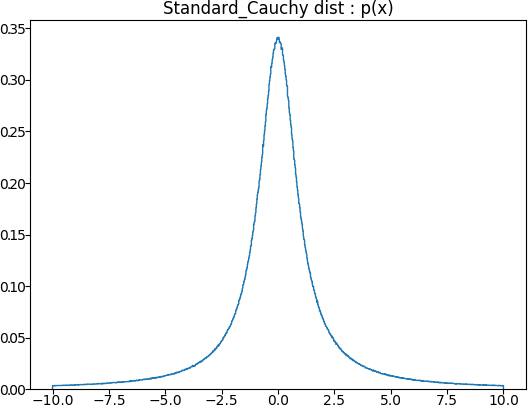
\includegraphics[clip, width=5cm]{../5/code/cauchy.png}
\end{center}
\end{figure}

ロングテール分布として有名.



\begin{itembox}[l]{較正}
…偏差の古典概念に対するベイズアナロジーである事後推論は事後平均の較正の概念を用いることで評価できる.
\end{itembox}


\begin{itembox}[l]{誤較正}
…任意のパラメータ$\theta$に対して, $\hat{\theta}=\text{E}(\theta|y)$とすると, $\text{E}(\theta|
\hat{\theta})-\hat{\theta}$として事後平均の\tcr{誤較正(miscalibration)}を定義する.
\end{itembox}

中心化のこと.


%==============================================================================================================%



%==============================================================================================================%



%==============================================================================================================%



%==============================================================================================================%



%==============================================================================================================%



%==============================================================================================================%



%==============================================================================================================%



%==============================================================================================================%



%==============================================================================================================%



%==============================================================================================================%



%==============================================================================================================%



%==============================================================================================================%



%==============================================================================================================%



%==============================================================================================================%



%==============================================================================================================%



%==============================================================================================================%



%==============================================================================================================%



%==============================================================================================================%



%==============================================================================================================%



%==============================================================================================================%



%==============================================================================================================%



%==============================================================================================================%



%==============================================================================================================%



%==============================================================================================================%



%==============================================================================================================%



%==============================================================================================================%



%==============================================================================================================%



%==============================================================================================================%



%==============================================================================================================%



%==============================================================================================================%



%==============================================================================================================%



%==============================================================================================================%



%==============================================================================================================%



%==============================================================================================================%



%==============================================================================================================%



%==============================================================================================================%



%==============================================================================================================%



%==============================================================================================================%



%==============================================================================================================%



%==============================================================================================================%



%==============================================================================================================%



%==============================================================================================================%



%==============================================================================================================%



%==============================================================================================================%



%==============================================================================================================%



%==============================================================================================================%



%==============================================================================================================%



%==============================================================================================================%



%==============================================================================================================%



%==============================================================================================================%



%==============================================================================================================%



%==============================================================================================================%



%==============================================================================================================%



%==============================================================================================================%



%==============================================================================================================%



%==============================================================================================================%



%==============================================================================================================%



%==============================================================================================================%



%==============================================================================================================%



%==============================================================================================================%



%==============================================================================================================%



%==============================================================================================================%



%==============================================================================================================%



%==============================================================================================================%



%==============================================================================================================%



%==============================================================================================================%



%==============================================================================================================%



%==============================================================================================================%



%==============================================================================================================%



%==============================================================================================================%



%==============================================================================================================%



%==============================================================================================================%



%==============================================================================================================%



%==============================================================================================================%



%==============================================================================================================%



%==============================================================================================================%



%==============================================================================================================%



%==============================================================================================================%



%==============================================================================================================%











\end{document}